\begin{frame}{CRUD in MongoDB (1): Via the shell}
  \begin{itemize}
      \item CRUD (Create, Read, Update, Delete) in MongoDB
        \inote{You need to be able to do something with the database}
      \item we will use the shell for now
        \inote{We will talk about integration into programming languages later}
      \item Queries themselves are JSON
        \inote{we use a version of javascript to specify the operation itself}
      \item enter them in an interactive shell
        \inote{the ``mongo'' executable}
  \end{itemize}
\end{frame}

\begin{frame}{CRUD in MongoDB (2): Selecting Database \& Collection}
  \begin{center}
    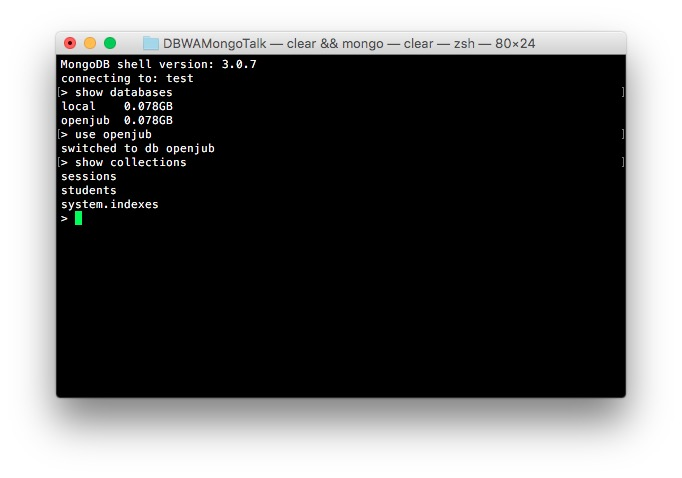
\includegraphics[width=0.80\textwidth]{imgs/shell_basic}\\\noindent
    \lstinline{show databases}, \\\noindent
    \lstinline{use some\_awesome\_database}, \\\noindent
    \lstinline{show collections}
  \end{center}
\end{frame}

\begin{frame}{CRUD in MongoDB (3): Find, insert, update, delete}
  \begin{center}
    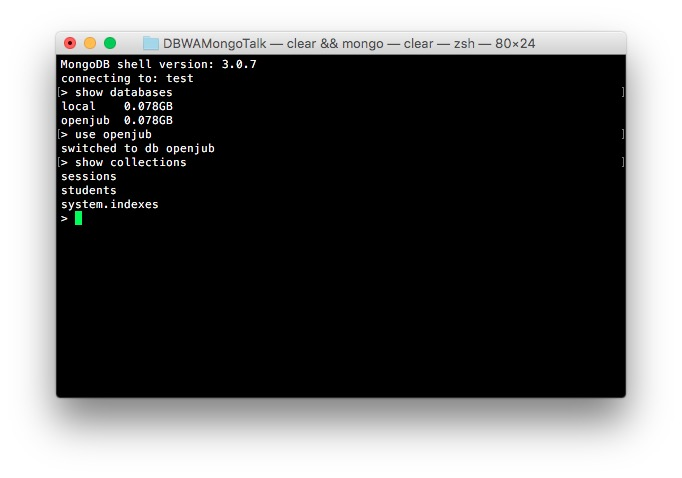
\includegraphics[width=0.80\textwidth]{imgs/shell_basic}\\\noindent
    \lstinline{db.my_collection.find(query)}, \\\noindent
    \lstinline{db.my_collection.insert(document)}, \\\noindent
    \lstinline{db.my_collection.update(query, change)}, \\\noindent
    \lstinline{db.my_collection.remove(query)}
  \end{center}
\end{frame}
